% !TeX spellcheck = pt_BR
\documentclass[tese_patricia]{subfiles}
\begin{document}

% ---------------------------------------------------------- 
% Métodos de malhas sobrepostas
% ----------------------------------------------------------
\chapter[Técnica de decomposição de domínios]{Técnica de decomposição de domínios} \label{capitulo:Cap4}
% ----------------------------------------------------------

Muitas aplicações de engenharia envolvem efeitos localizados, são os casos, por exemplo, de fissuras na mecânica dos sólidos, interface entre dois tipos diferentes de fluidos na mecânica dos fluidos, ou ainda, a camada limite na interface entre sólido e fluido, entre outros. Para uma análise computacional realística desses problemas, os efeitos locais devem ser apropriadamente representados e a um custo computacional razoável. 

Neste trabalho aplica-se um método decomposição de domínios que permite utilizar uma malha local mais refinada sobreposta a uma malha global com discretização mais grosseira com o intuito de melhorar a precisão local da análise numérica ou simplesmente representar a geometria local e as condições de contorno adequadamente. A malha local pode ter uma escala diferente de discretização, ou até mesmo uma aproximação numérica diferente, como no caso deste trabalho em que se utiliza o método dos elementos finitos em conjunto com a análise isogeométrica.

\section{Combinação de espaços de funções}

Para o entendimento da técnica de sobreposição de malhas define-se inicialmente um dom\'inio global $\Omega_G$, de acordo com a Fig. \ref{fig:global_domain}, e um dom\'inio local, $\Omega_L$, apresentado na Fig. \ref{fig:local_domain}, menor que o dom\'inio global e que cont\'em a regi\~ao com efeitos localizados. O dom\'inio total de estudo \'e ent\~ao composto por: $\Omega = \Omega_G \cup \Omega_L$.

Adicionalmente definem-se os contornos desses dom\'inios, conforme Fig. \ref{fig:overlap_domain}, como: $\Gamma_{G}$ contorno f\'isico de $\Omega$ determinado pelo dom\'inio global; $\Gamma_{L}$ contorno f\'isico de $\Omega$ pertencente ao dom\'inio local; $(\Gamma_{G})_{B}$ contorno que define a regi\~ao de sobreposi\c{c}\~ao pertencente ao dom\'inio global e $(\Gamma_{L})_{B}$ contorno que define a regi\~ao de sobreposi\c{c}\~ao pertencente ao dom\'inio local. \'E importante observar que os dom\'inios ditos f\'isicos podem ou n\~ao estarem presentes nos problemas de sobreposi\c{c}\~ao. A zona dita de sobreposi\c{c}\~ao $\Omega_{B} = \Omega_G \cap \Omega_L$ \'e definida pelos contornos $(\Gamma_{L})_{B}$ e $(\Gamma_{G})_{B}$.


\begin{figure}[!htb]
	\centering
	\subfloat[\label{fig:global_domain} Domínio Global]{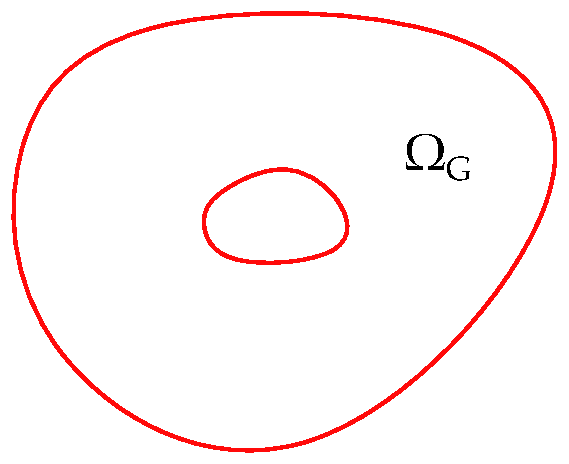
\includegraphics[scale=0.6,trim=0cm 0cm 0cm 0cm, clip=true]{Imagens/Cap4/dominioglobal.pdf}} 
	\subfloat[\label{fig:local_domain} Domínio Local]{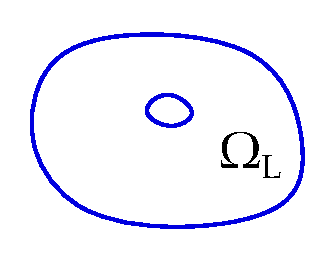
\includegraphics[scale=0.6,trim=0cm 0cm 0cm 0cm, clip=true]{Imagens/Cap4/dominiolocal.pdf}} \\
	\subfloat[\label{fig:overlap_domain} Domínios sobrepostos]{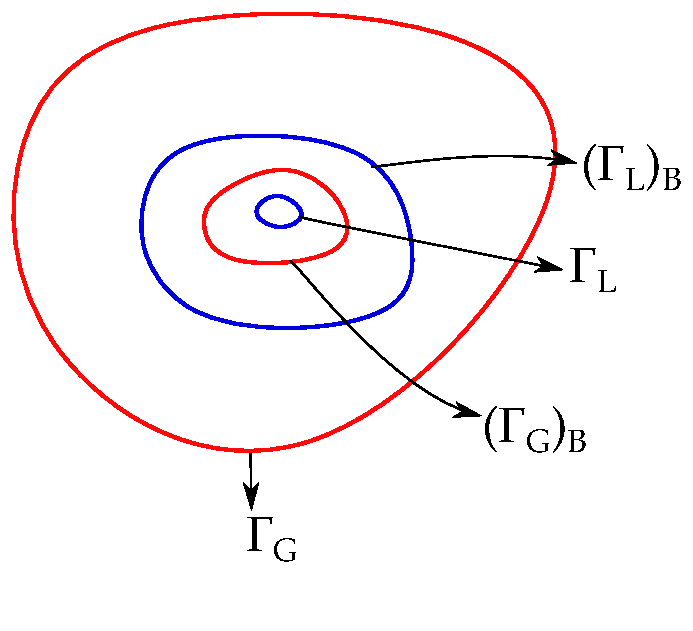
\includegraphics[scale=0.6,trim=0cm 0cm 0cm 0cm, clip=true]{Imagens/Cap4/dominiosobreposto.pdf}} 
	\caption{Definição dos domínios global,local e de sobreposição. }
	\label{fig:domains}
\end{figure}

O espa\c{c}o de fun\c{c}\~oes tentativa global $u_{G}(\mathbf{x})$ \'e definido como $\usolution^{G}$, e o espa\c{c}o das fun\c{c}\~oes tentativa local $u_{L}(\mathbf{x})$ por $\usolution^{L}$, com funções peso global $w_{G}(\mathbf{x})$ e local $w_{L}(\mathbf{x})$ definidas nos espa\c{c}o $\uweighting^{G}$ e $\uweighting^{L}$ respectivamente. A uni\~ao direta dos espaços de funções na zona de sobreposição obviamente não resulta em um espaço que respeita a partição da unidade. 
Dessa forma, utiliza-se uma fun\c{c}\~ao ponderadora de combinação $b(\mathbf{x})$, de maneira a criar um novo espaço de funções tentativa e peso definidas por:

\begin{align}
u(\mathbf{x}) = b(\mathbf{x})u_{G}(\mathbf{x}) + (1-b(\mathbf{x}))u_{L}(\mathbf{x}),\\
w(\mathbf{x}) = b(\mathbf{x})w_{G}(\mathbf{x}) + (1-b(\mathbf{x}))w_{L}(\mathbf{x}),
\end{align}

\noindent com a função $b(\mathbf{x})$ apresentando valor unitário sobre o domínio global livre (sem sobreposições), e valor zero no domínio local livre, e com uma transição suave na região de sobreposição. 

Os espaços enriquecidos na região de sobreposição de malhas, s\~ao definidos por $\mathcal{S}_{enr}^{h}$ e $\mathcal{V}_{enr}^{h}$, correspondentes às fun\c{c}\~oes tentativa e teste respectivamente. A solu\c{c}\~ao de um problema de valor de contorno recai em encontrar $u^{h} \in \mathcal{S}_{enr}^{h}$ tal que $\forall$ $ w^{h} \in \mathcal{V}_{enr}^{h}$: 

\begin{align}
B(u^{h},w^{h}) = F(w^{h}),
\end{align}

\noindent com $B(\bullet,\bullet)$ e $F(\bullet)$ sendo operadores bilineares e lineares respectivamente. A discretiza\c{c}\~ao de $u(\mathbf{x})$ e $w(\mathbf{x})$ no contexto dos elementos finitos \'e obtida atrav\'es das seguintes rela\c{c}\~oes:

\begin{align}
u^{h}(\mathbf{x}) = \sum_{A = 1}^{(n_{np})_G} (u_{G})_{A}b(\mathbf{x})(N_{G})_{A}(\mathbf{x}) + \sum_{A = 1}^{(n_{np})_L} (u_{L})_{A}(1-b(\mathbf{x}))(N_{L})_{A}(\mathbf{x}),\\
w^{h}(\mathbf{x}) = \sum_{A = 1}^{(n_{np})_G} (w_{G})_{A}b(\mathbf{x})(N_{G})_{A}(\mathbf{x}) + \sum_{A = 1}^{(n_{np})_L} (w_{L})_{A}(1-b(\mathbf{x}))(N_{L})_{A}(\mathbf{x}),
\end{align}

\noindent com $N_{G}$ e $N_{L}$ sendo as fun\c{c}\~oes de forma global e local; e $(n_{np})_G$ e $(n_{np})_L$ o n\'umero de fun\c{c}\~oes de forma nas discretiza\c{c}\~oes global e local respectivamente. 

\subsection{Função ponderadora de combinação}

De maneira a se obter uma solu\c{c}\~ao  \'unica deseja-se que as fun\c{c}\~oes $b(\mathbf{x})(N_{G})$ e $(1-b(\mathbf{x}))(N_{L})$ sejam linearmente independentes sobre $\Omega_{B}$. Esta não é uma questão simples de ser garantida de forma geral. Considerando que as fun\c{c}\~oes base local e global possuem grau polinomial $p$ e s\~ao linearmente independentes, e que $b(\mathbf{x})$ e $(1-b(\mathbf{x}))$ s\~ao linearmente independentes, adota-se $b(\mathbf{x})$ com grau polinomial 1 vez superior as fun\c{c}\~oes base ($p+1$). Isso resulta um espaço enriquecido onde o número de funções de forma em cada ponto da zona de superposição é compatível com o grau do polinômio.  

Nesse trabalho aplicam-se funções de forma locais e globais de grau polinomial quadrático. Dessa forma, a função de combinação foi definida como cúbica e é expressa por:

\begin{align}
b(\mathbf{x}) =  \begin{cases} 2\left(\frac{X_{L}(\mathbf{x})}{\delta\mathbf(x)}\right)^3  -   3\left(\frac{X_{L}(\mathbf{x})}{\delta\mathbf(x)}\right)^2   \mbox{se } X_{G}(\mathbf{x})> 0 \ e \ X_{L}(\mathbf{x})> 0 \\
1  \ X_{L}(\mathbf{x}) \leq 0  \\
0  \ X_{G}(\mathbf{x}) \leq 0 \end{cases},
\end{align}

\noindent com $X_{L}(\mathbf{x})$ a função distância assinalada medida a partir de $(\Gamma_{L})_{B}$, com valores positivos dentro do domínio local e negativos fora, e $X_{G}(\mathbf{x})$ a função distância assinalada medida a partir de $(\Gamma_{G})_{B}$, sendo positivo se o ponto pertence à $\Omega_{G}$ e negativos caso contr\'ario. Nota-se que os pontos em que ambas funções distância assinalada são positivos estão contidos dentro da zona de sobreposição. O parâmetro $\delta$ \'e obtido por $\delta(\mathbf{x}) = X_{L}(\mathbf{x}) + X_{G}(\mathbf{x})$, e coincide com a espessura da zona de sobreposi\c{c}\~ao quando $(\Gamma_{L})_{B}$ e $(\Gamma_{G})_{B}$ s\~ao paralelos.

Na pr\'atica, considera-se que o dom\'inio global tem o tamanho do dom\'inio total, ficando a defini\c{c}\~ao de $(\Gamma_{G})_{B}$ para uma etapa posterior, baseado na forma do modelo local, e os elementos e n\'os sem suporte f\'isico ap\'os a obten\c{c}\~ao do novo espa\c{c}o de fun\c{c}\~oes s\~ao desativados da an\'alise.

O contorno $(\Gamma_{G})_{B}$ pode ser obtido atrav\'es de uma r\'eplica do contorno $(\Gamma_{L})_{B}$ a uma dist\^ancia paralela $\delta$ do mesmo.  Na Fig. \ref{fig:ZonadeSobreposicao} apresenta-se um exemplo do espaço de funções obtido para um caso unidimensional a partir de funções base Lagrangianas quadráticas para os domínios global e local.


\begin{figure}[!htb]
	\centering
	\subfloat[\label{fig:overlap1} Funções Globais e função ponderadora ($b$).]{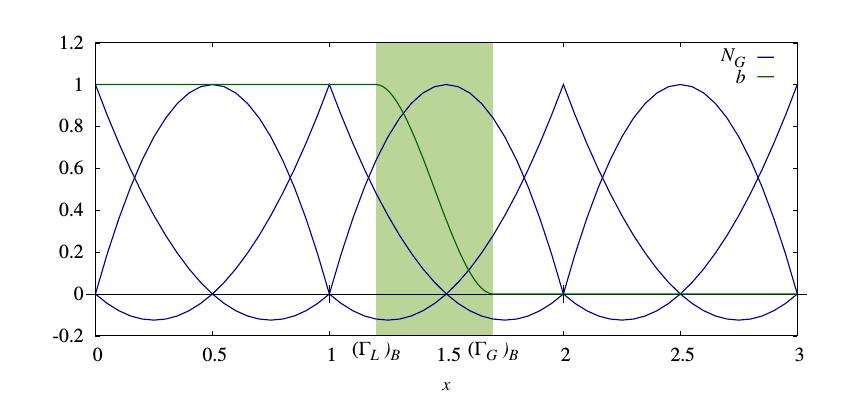
\includegraphics[scale=0.4, trim=0cm 0cm 0cm 0cm, clip=true]{Imagens/Cap4/Overlap1.png}} \\
	\subfloat[\label{fig:verlap2} Funções locais e função ponderadora ($1-b$) ]{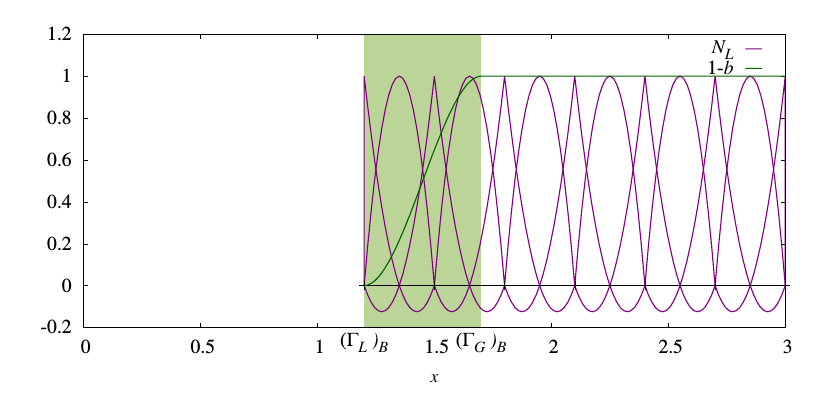
\includegraphics[scale=0.4,trim=0cm 0cm 0cm 0cm, clip=true]{Imagens/Cap4/Overlap2.png}} \\
	\subfloat[\label{overlap3} Novo espaço de funções]{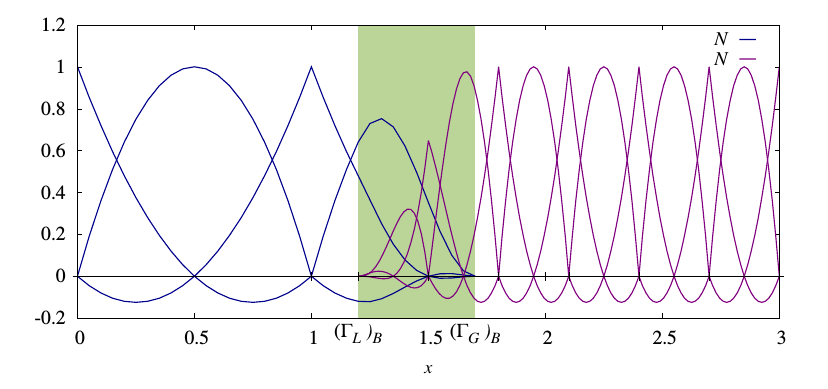
\includegraphics[scale=0.4,trim=0cm 0cm 0cm 0cm, clip=true]{Imagens/Cap4/Overlap3.png}} 
	\caption{Zona de sobreposição - Problema unidimensional. }
	\label{fig:ZonadeSobreposicao}
\end{figure}


Após a definição $(\Gamma_{G})_{B}$ é necessária uma metodologia eficiente para determinação das funções base globais com pequena influência dentro da zona de sobreposição, visto que essas podem levar a um sistema mal condicionado. Para resolver esse problema, utiliza-se, para todos os n\'os globais A da análise, uma variável definida como:

\begin{align}
(M_{G})_{AA} = \int_{\Omega}b(\bm{\xi})N_{A}(\bm{\xi})b(\bm{\xi})N_{A}(\bm{\xi})d\Omega, \label{eq:influence}
\end{align}

\noindent e define-se um valor $M_{min}$ para $(M_{G})_{AA}$. Os n\'os globais s\~ao desativados se $(M_{G})_{AA} < M_{min}$.

Os parâmetros de estabilização utilizados nesta formulação ainda necessitam um estudo mais aprofundado. No presente trabalho, faz-se a combinação dos parâmetros calculados em cada discretização:

\begin{align}
\SUPG(\mathbf{x}) =  b(\mathbf{x})\SUPG^{G}(\mathbf{x}) + (1-b(\mathbf{x}))\SUPG^{L}(\mathbf{x}),\\
\PSPG(\mathbf{x}) =  b(\mathbf{x})\PSPG^{G}(\mathbf{x}) + (1-b(\mathbf{x}))\PSPG^{L}(\mathbf{x}),\\
\LSIC(\mathbf{x}) =  b(\mathbf{x})\LSIC^{G}(\mathbf{x}) + (1-b(\mathbf{x}))\LSIC^{L}(\mathbf{x}),
\end{align}

\noindent com $\SUPG^{G}$, $\PSPG^{G}$ e $\LSIC^{G}$ sendo os parâmetros de estabilização na malha global e $\SUPG^{L}$, $\PSPG^{L}$ e  $\LSIC^{L}$ sendo os parâmetros de estabilização na malha local.


\section{Implementação Computacional}

O algoritmo de partição de domínios foi implementado para a solução de escoamentos incompressíveis seguindo a formulação apresentada nos capítulos \ref{capitulo:Cap1} e \ref{capitulo:Cap2}. Nesse código, após a leitura dos dados respectivos às malhas global e local, segue-se com a definição da distância assinalada respectiva a todos os nós da malha global e da malha local com respeito aos contornos $(\Gamma_{G})_{B}$ e $(\Gamma_{L})_{B}$. O contorno  $(\Gamma_{G})_{B}$ é obtido a partir dos dados de entrada, onde define-se a espessura da zona de sobreposição. De posse da distância assinalada e espessura da zona de sobreposição, são definidos quais elementos das malhas local e global fazem parte da zona de sobreposição. Qualquer elemento que possua 1 ou mais nós dentro da zona de sobreposição é considerado como um elemento pertencente a ela.

As equações na região de sobreposição são integradas sobre o elemento local, dessa forma, num processo prévio à solução, os pontos de integração da malha local são projetados sobre a malha global e o elemento e coordenadas locais a que pertencem são armazenados. 

Determinam-se também os nós inativos da malha global, sejam porque encontram-se fora da zona de sobreposição, ou, porque possuem pequena influência dentro da mesma, de acordo com a Eq. \ref{eq:influence}.

Finalmente, o processo de marcha no tempo se inicia da maneira explicitada no Item \ref{subsection:DFCComputationalCode} levando-se em consideração que as funções tentativa e peso, e os parâmetros de estabilização são modificados de acordo com o apresentado neste capítulo.

O algoritmo que descreve esse processo de solução das equações da DFC considerando a partição de domínios pode ser visualizado no Alg. \ref{alg:overlap}.


\begin{algorithm}
	\caption{Algoritmo para problemas de dinâmica dos fluidos computacional com sobreposição de malhas}
	\label{alg:overlap}
	\begin{algorithmic}[1]
		\State Cálculo da distância assinalada dos nós e pontos de controle aos contornos;
		\State Determinação dos elementos e células da zona de sobreposição;
		\State Busca dos pontos de integração na malha global equivalentes aos definidos para à malha local;
		\State Definição dos nós inativos da malha global;
		\For {o passo de tempo $0$ até \timeInterval} 
		\State $i=0$;
		\State Predição da solução: aplicação das Eq. \eqref{eq:Pred1}, Eq. \eqref{eq:Pred2} e Eq. \eqref{eq:Pred3};
		\While{($\epsilon$ < tolerância)}
		\State $i$++;
		\State Interpolação das variáveis do problema: aplicação da Eq. \eqref{eq:approx_accelerationI}, Eq. \eqref {eq:approx_velocityI} e Eq. \eqref{eq:approx_pressI};
		\State Cálculo do incremento nas variáveis do problema: $\Acceleration_{n+1}$ e $\Press_{n+1}$ de acordo com as Eq. \eqref{eq:NR1} e Eq. \eqref{eq:NR2};
		\State Atualização da solução: calculadas de acordo com Eq. \eqref{update1}, Eq. \eqref{update2} e Eq. \eqref{update3}.
		\State Cálculo do erro:
		\begin{align}
		\epsilon =\left\| \NNSM^i \right\|_{L^2}
		\end{align}
		\EndWhile
		\EndFor
	\end{algorithmic}
\end{algorithm}


\section{Exemplo de aplicação}

Para verificar a metodologia de partição de domínios com sobreposição de malhas, neste item apresenta-se a solução estacionária do problema de Navier Stokes para a cavidade 2D.

A geometria do problema e suas condições contorno são apresentadas na Fig. \ref{fig:CavBoundary}. O problema foi avaliado para um número de Reynolds = 100, calculado de acordo com Eq. \eqref{eq:Reynolds} e $\rho = 1,0$.

\begin{figure}[!htb]
	\centering
	{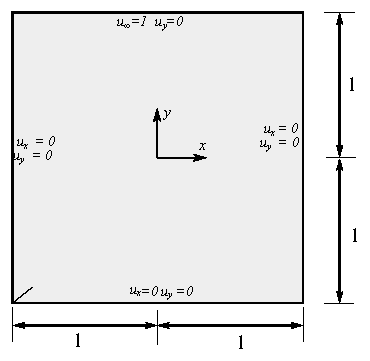
\includegraphics[scale=1.3,trim=0cm 0cm 0cm 0cm, clip=true]{Imagens/Cap4/cavidade.pdf}}
	\caption{Cavidade 2D: Condições de contorno.} 
	\label{fig:CavBoundary}
\end{figure}

Sabe-se que nas paredes da cavidade podem haver efeitos de camada limite, dessa forma, definiu-se uma malha local que circunda a cavidade de acordo com a Fig. \ref{fig:CavLocal}. A malha local foi discretizada através de uma aproximação isogeométrica e foi definida com 1440 pontos de controle que foram divididos em 8 diferentes \textit{patches}, chamados de $P_{1},P_{2},...,P_{8}$. Os \textit{patches} $P_{1},P_{3},P_{6}$ e $P_{6}$ possuem 64 células e os $P_{2},P_{4},P_{5}$ e $P_{7}$ 192 células.

A malha global por sua vez é definida para toda a seção da cavidade, sendo composta por 800 elementos triangulares quadráticos e 1681 nós, de acordo com Fig. \ref{fig:CavGlobal}.


\begin{figure}[!htb]
	\centering
	\subfloat[\label{fig:CavLocal} Malha Local.]{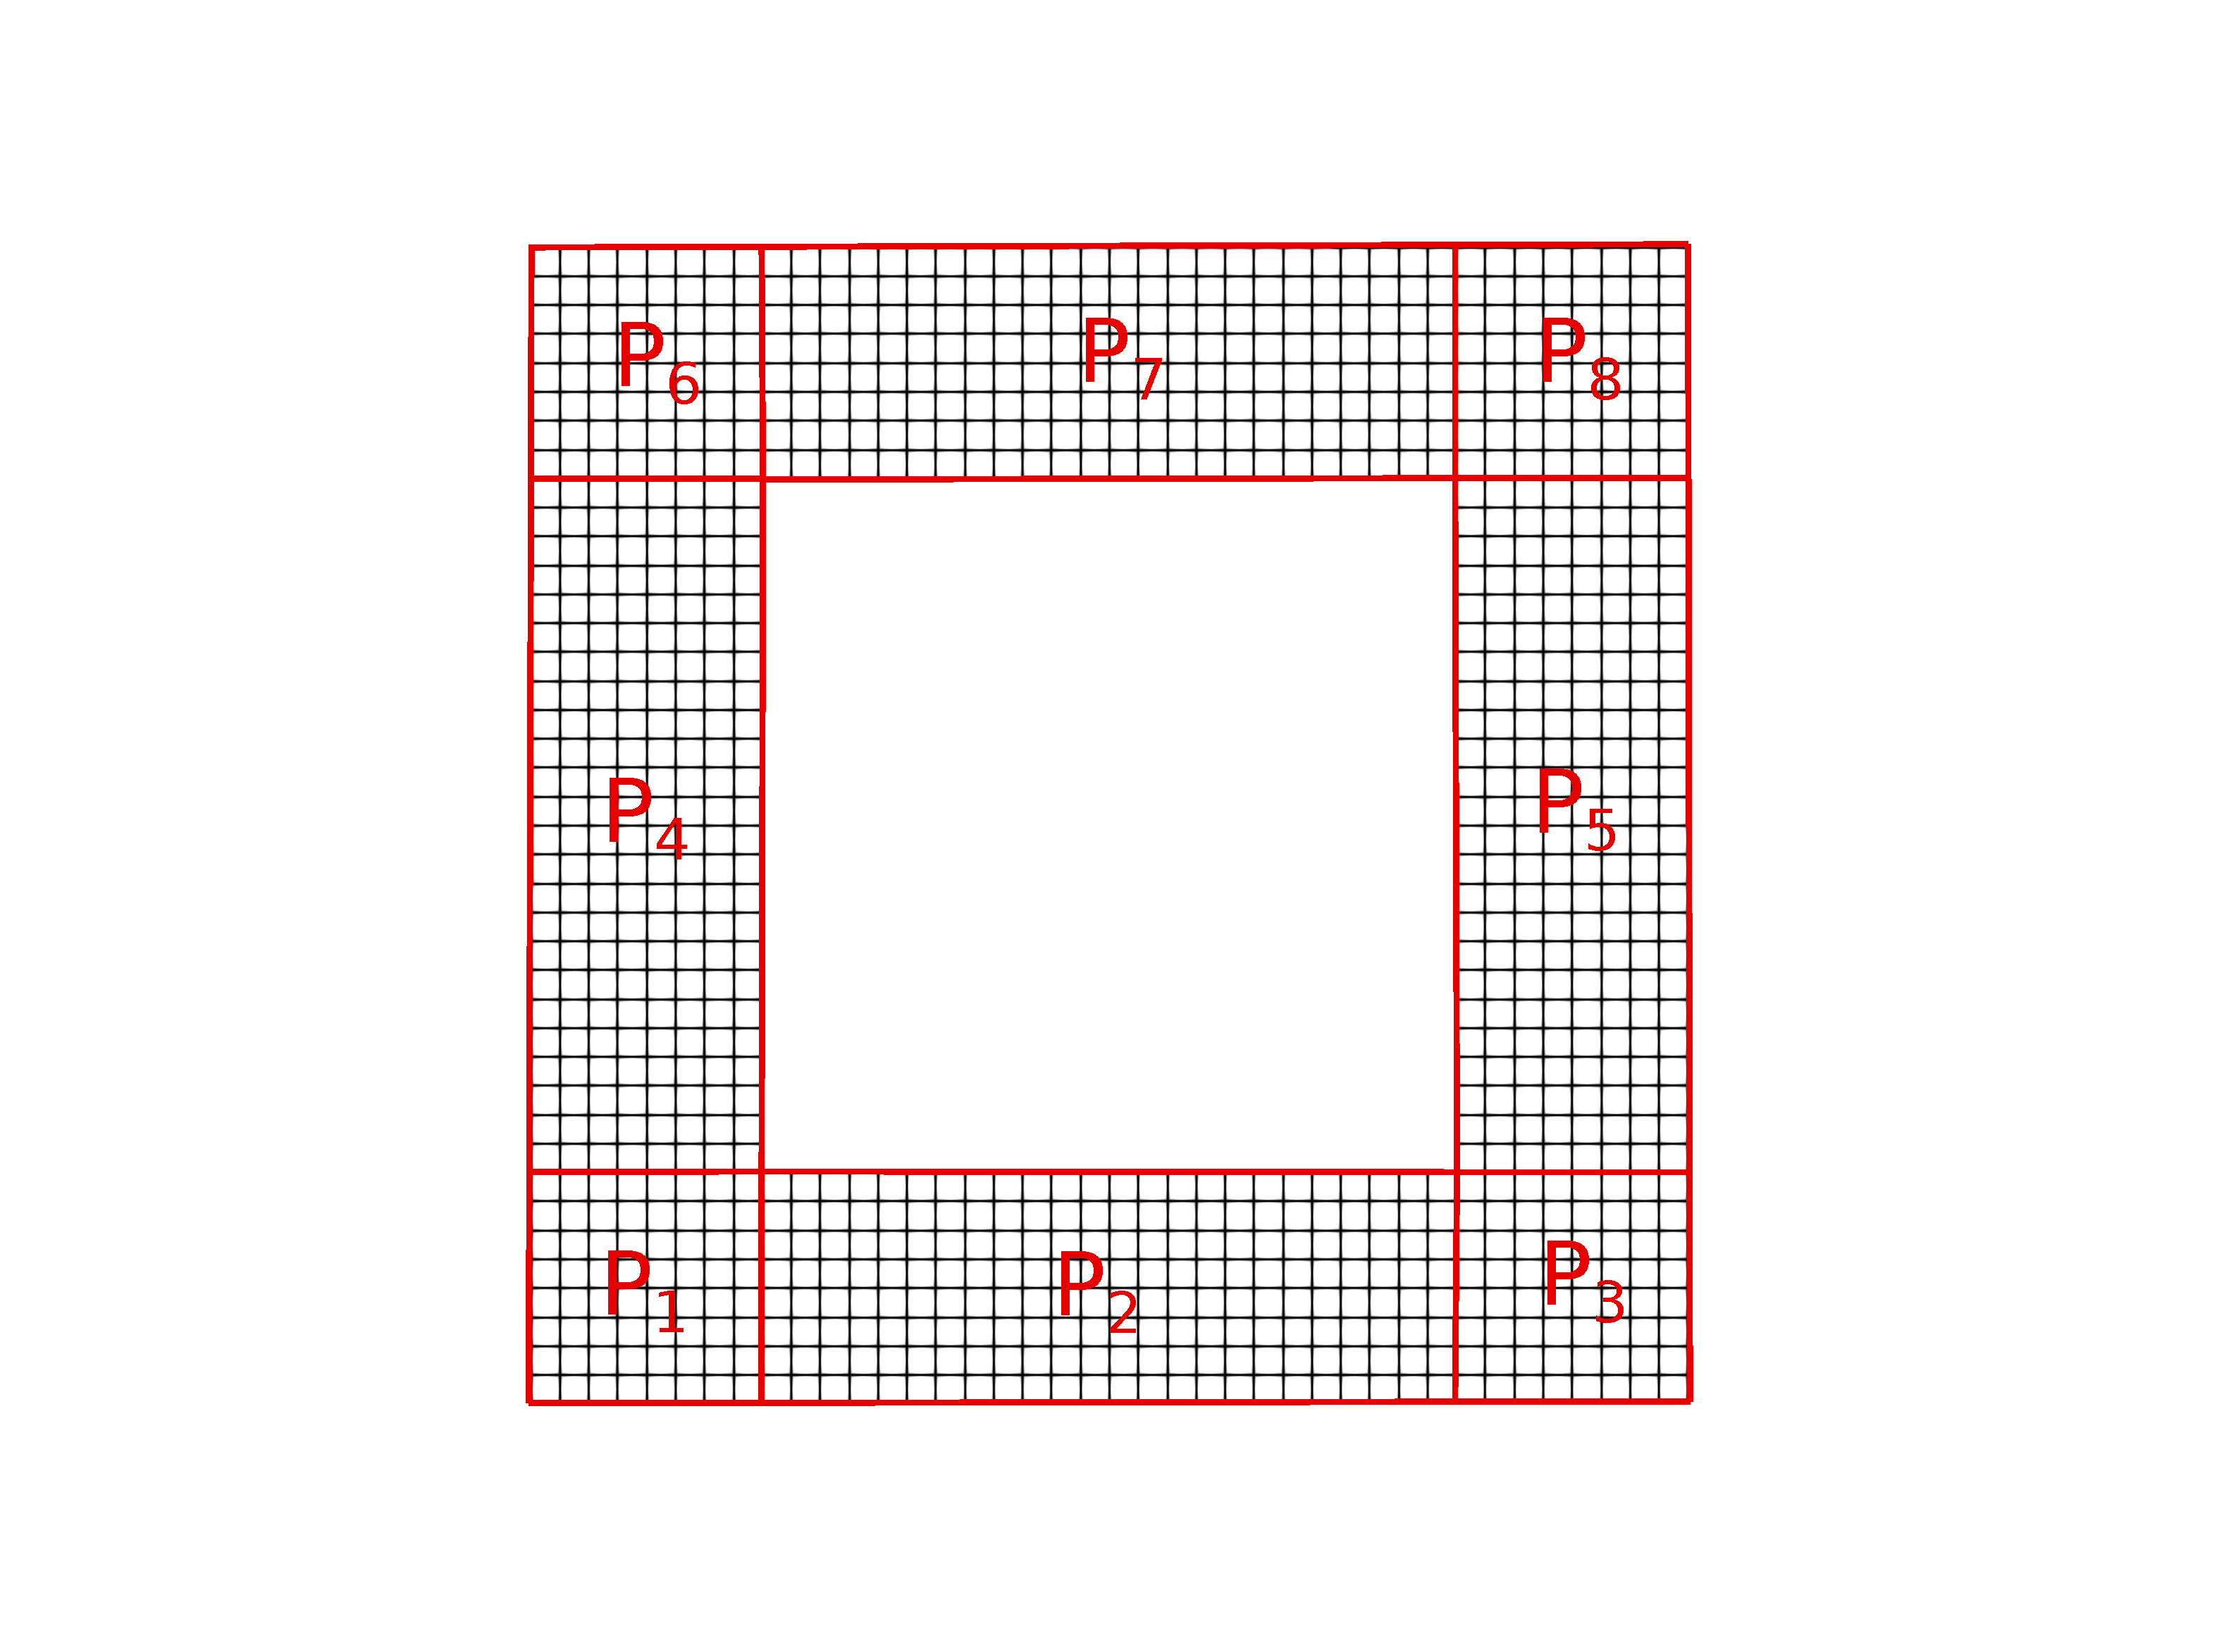
\includegraphics[scale=0.2, trim=9cm 3cm 9cm 3cm, clip=true]{Imagens/Cap4/malhaLocal.pdf}} 
	\subfloat[\label{fig:CavGlobal} Malha Global ]{\includegraphics[scale=0.15,trim=9cm 3cm 9cm 3cm, clip=true]{Imagens/Cap4/malhaGlobal.png}}
	\caption{Cavidade 2D: Malhas Global e Local.}
	\label{fig:CavOverlap}
\end{figure}

Definiu-se uma espessura para a zona de sobreposição de 0,1 medida paralelamente ao contorno fictício local $(\Gamma_{L})_{B}$, e, a partir desse dado, os elementos globais sob o domínio local $(\Omega_{L})$ e fora da zona de sobreposição $(\Omega_{B})$ foram desativados. As células e elementos pertencentes à zona de sobreposição, tanto para a malha local quanto para a malha global, podem ser vistos nas Fig. \ref{fig:blendzoneLocal} e Fig. \ref{fig:blendzoneGlobal} respectivamente.

\begin{figure}[!htb]
	\centering
	\subfloat[\label{fig:blendzoneLocal} Malha Local]{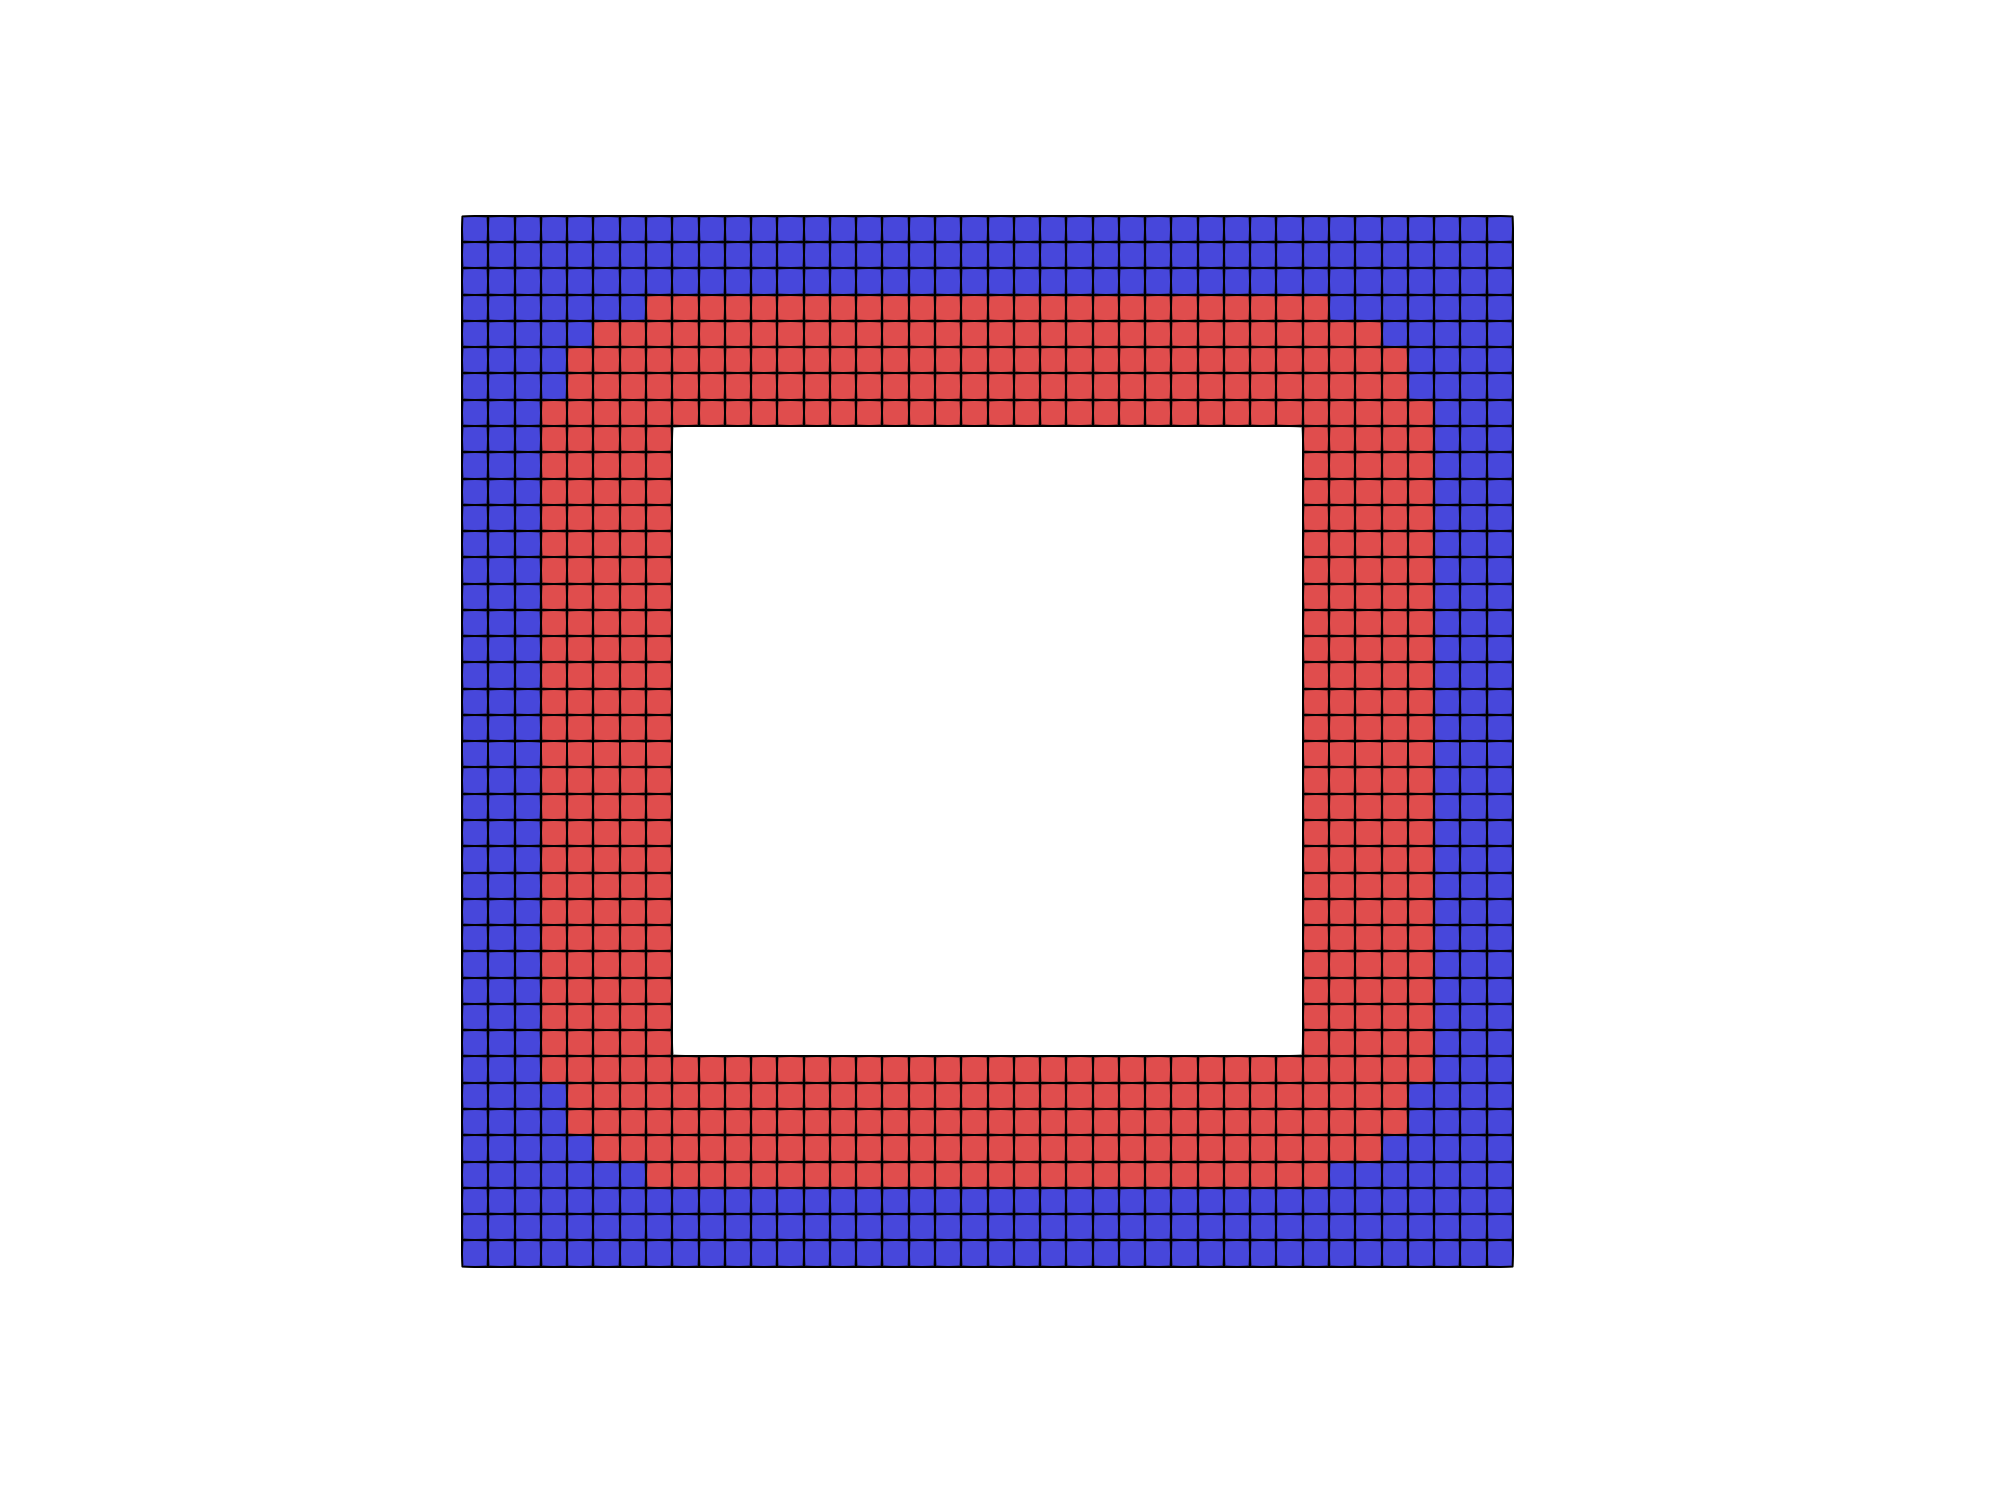
\includegraphics[scale=0.15, trim=9cm 3cm 9cm 3cm, clip=true]{Imagens/Cap4/blendzone.png}} 
	\subfloat[\label{fig:blendzoneGlobal} Malha Global ]{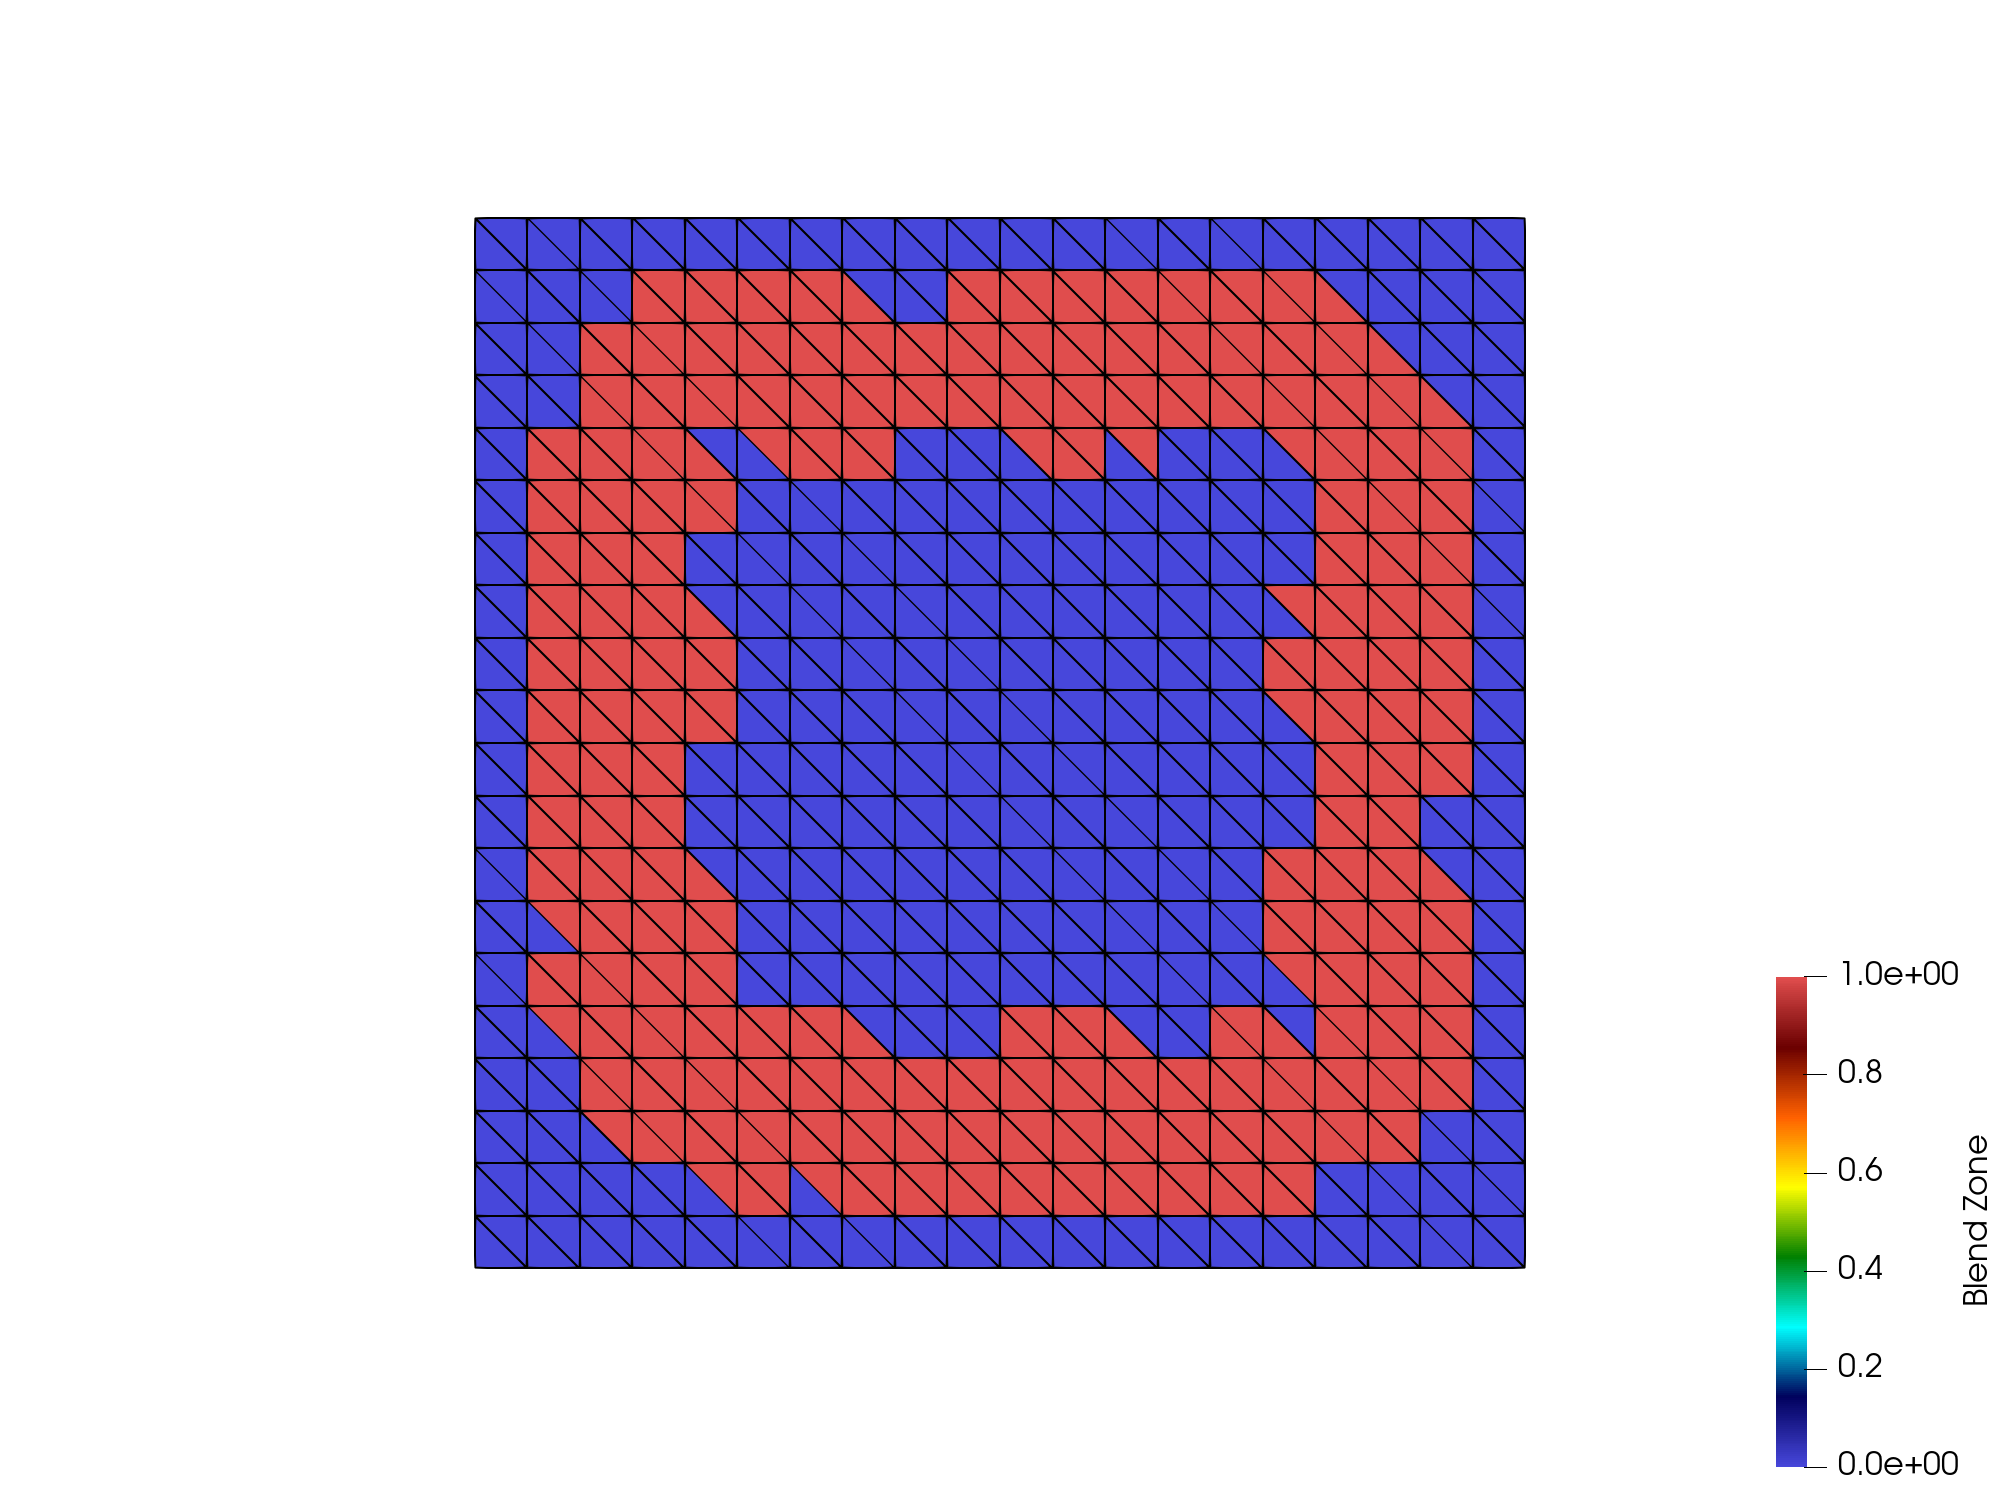
\includegraphics[scale=0.15,trim=9cm 3cm 9cm 3cm, clip=true]{Imagens/Cap4/blendzoneMG.png}}]]
    \caption{Cavidade 2D: Zona de sobreposição.}
	\label{fig:OverlapRegion}
\end{figure}

Os campos de velocidade e pressão obtidos são apresentados nas Fig. \ref{fig:CampoVelocidade} e Fig. \ref{fig:CampoPressao}.

\begin{figure}[!htb]
	\centering
	\subfloat[\label{fig:CampoVelocidade} Campo de Velocidade]{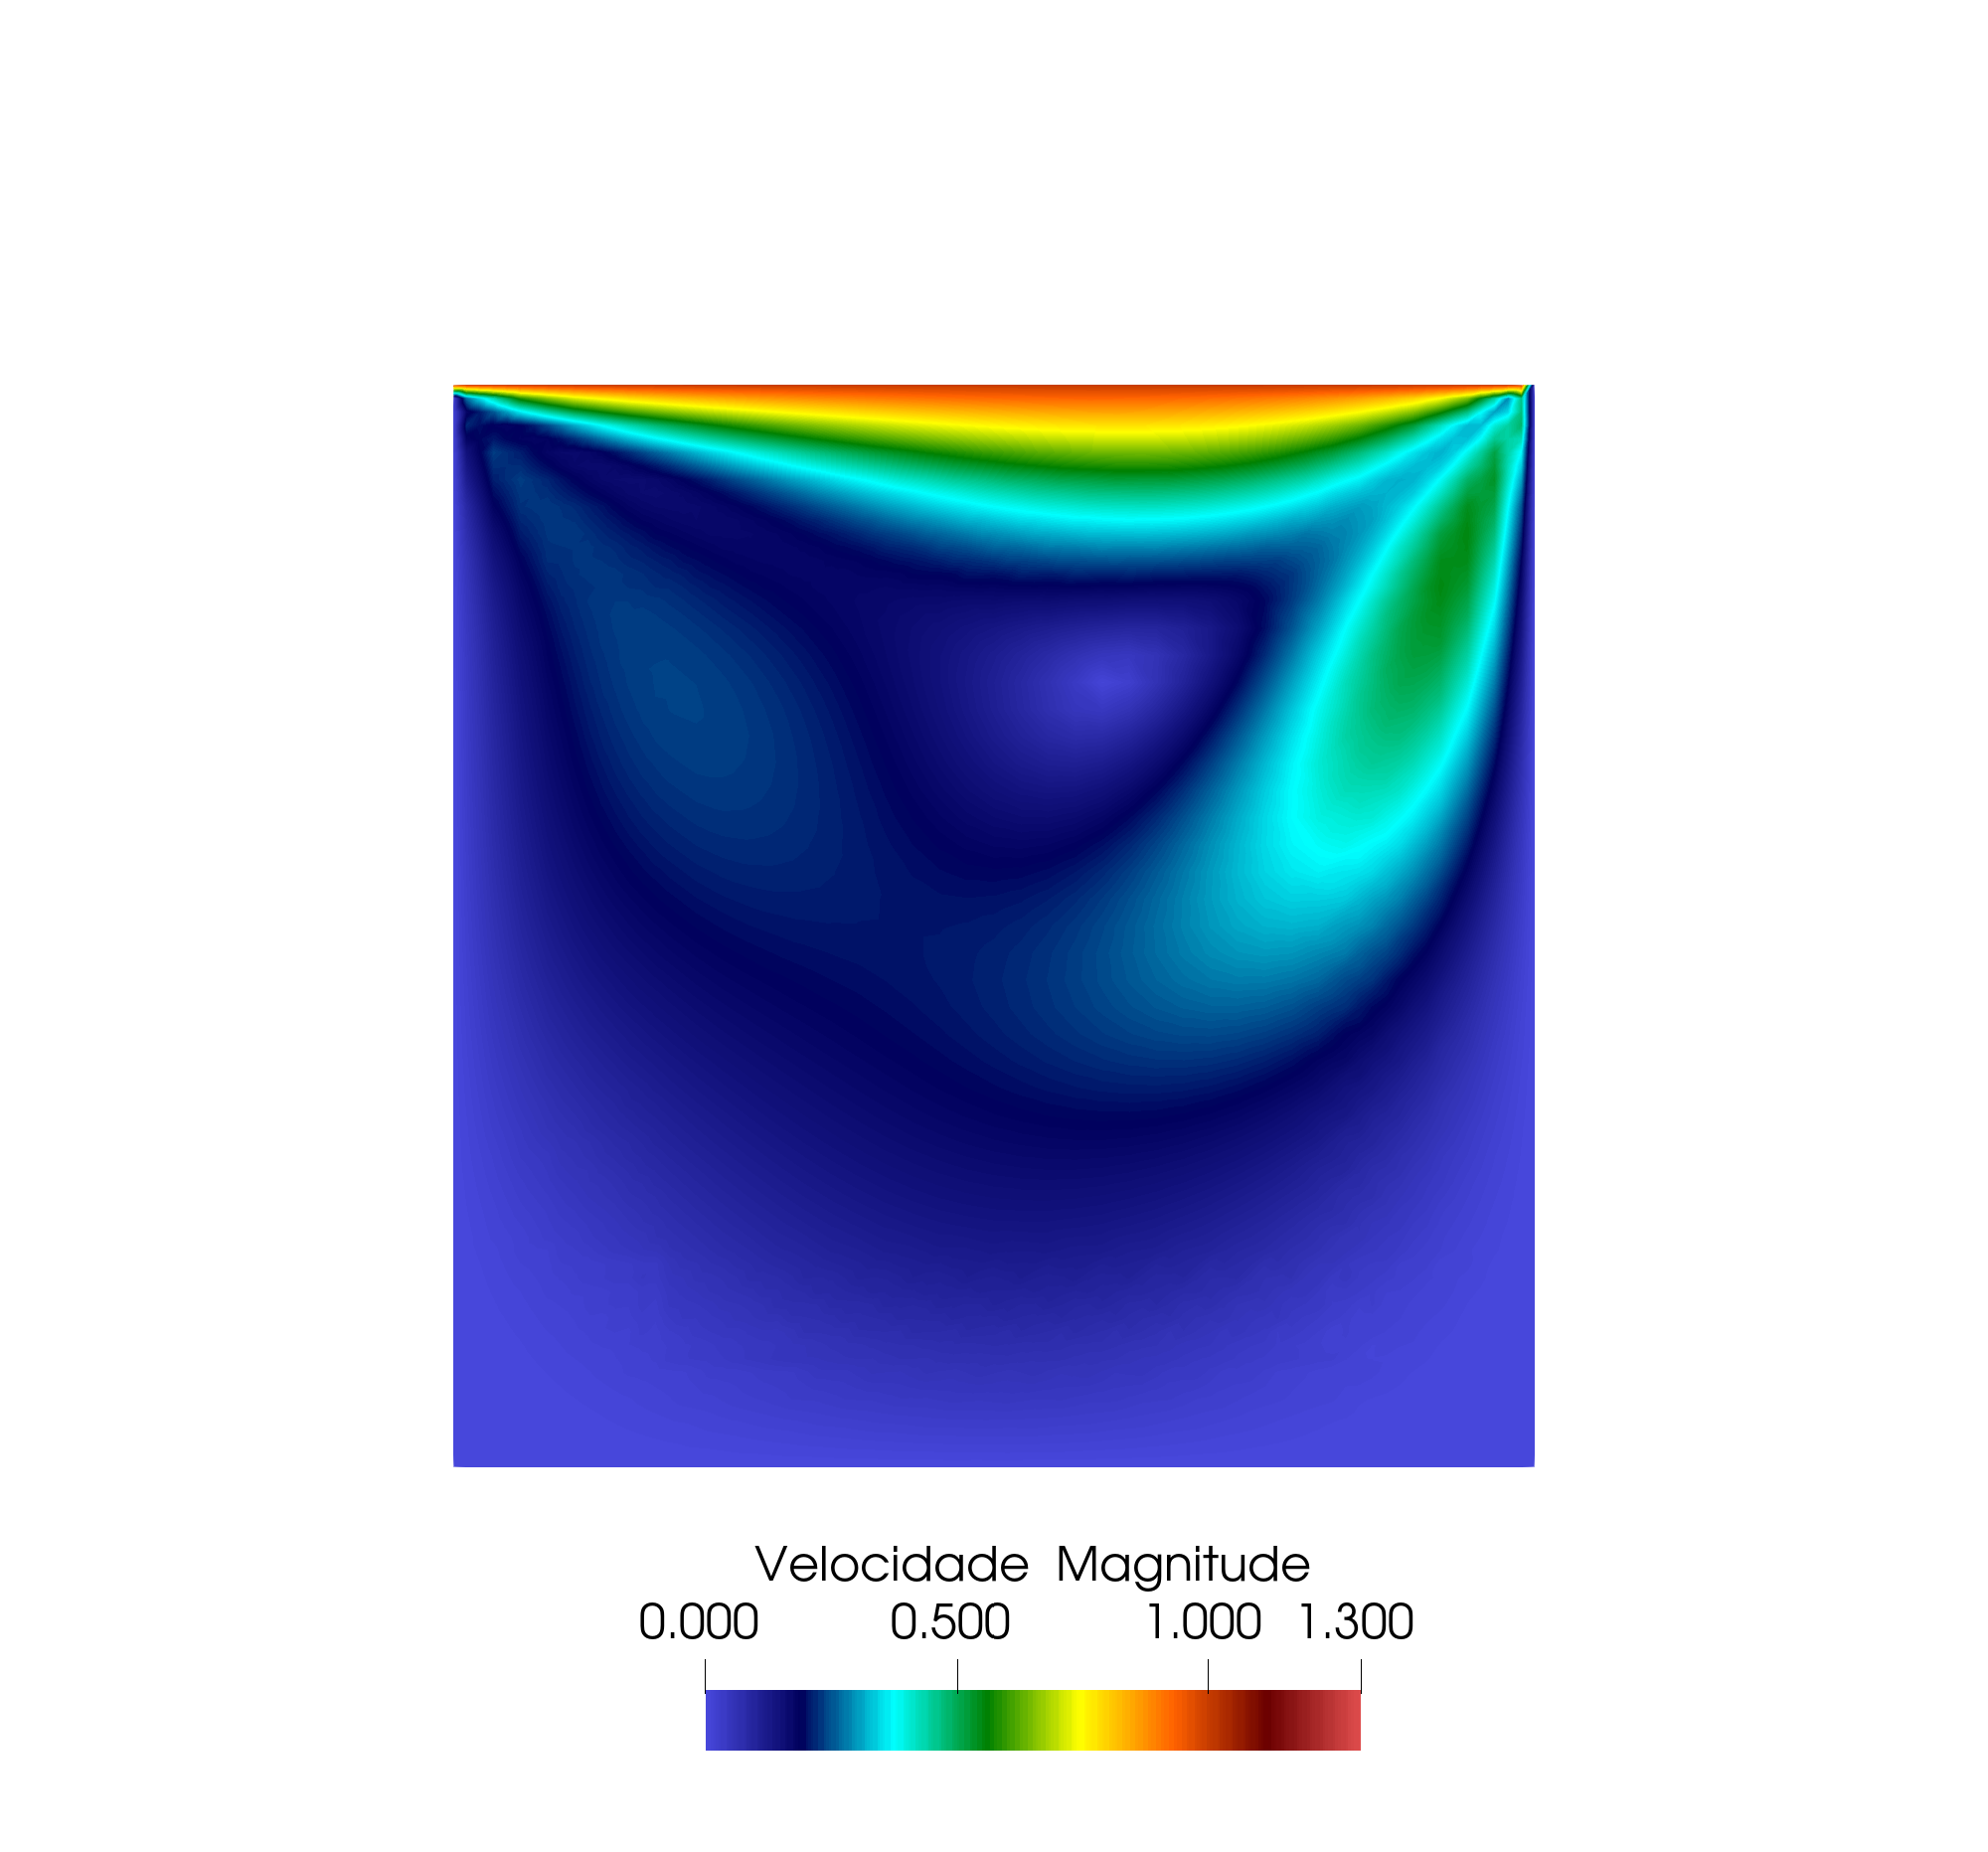
\includegraphics[scale=0.15, trim=9cm 3cm 9cm 3cm, clip=true]{Imagens/Cap4/VelocityMagnitude.png}} 
	\subfloat[\label{fig:CampoPressao} Campo de Pressão ]{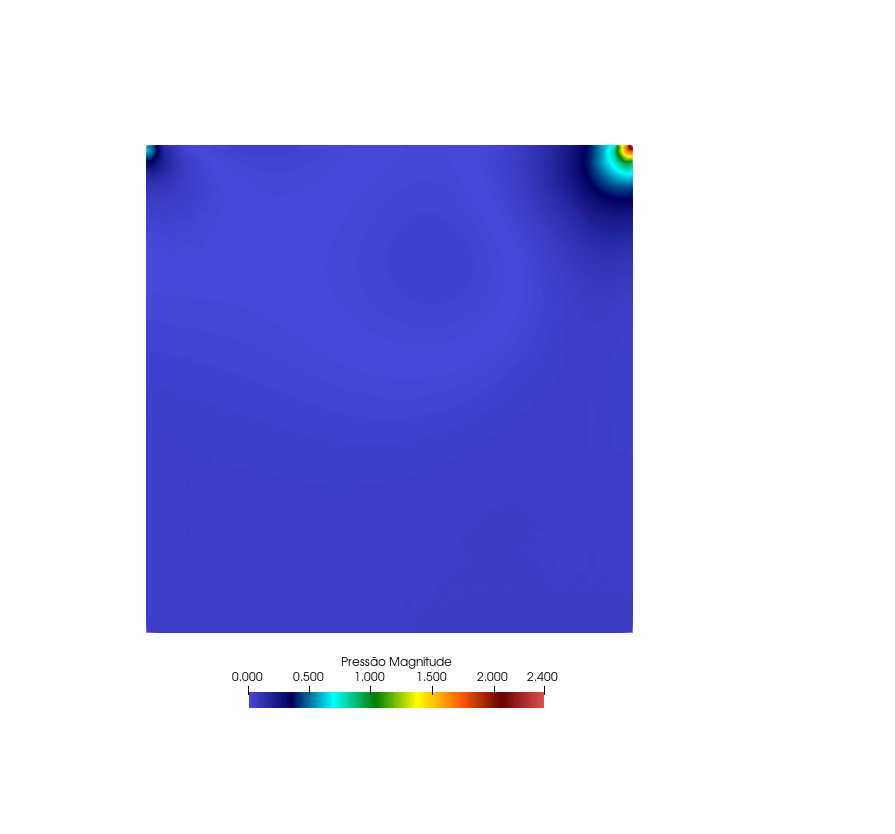
\includegraphics[scale=0.34,trim=0cm 3cm 6cm 0cm, clip=true]{Imagens/Cap4/PressureMagnitude.png}}
	\caption{Cavidade 2D: Solução do problema de Navier Stokes para $Re = 100$.}
	\label{fig:RespostasOverlap}
\end{figure}

Os perfis de velocidade adimensionalizados ($\velocity/\velocinfty$) horizontal e vertical ao longo de duas linhas centrais nas direções $x$ e $y$ da cavidade são apresentados na Fig. \ref{fig:cavidade_graficos_overlap} e comparados com os resultados de \citeonline{GhiaGS:1982}.

\begin{figure}[!htb]
	\centering
	{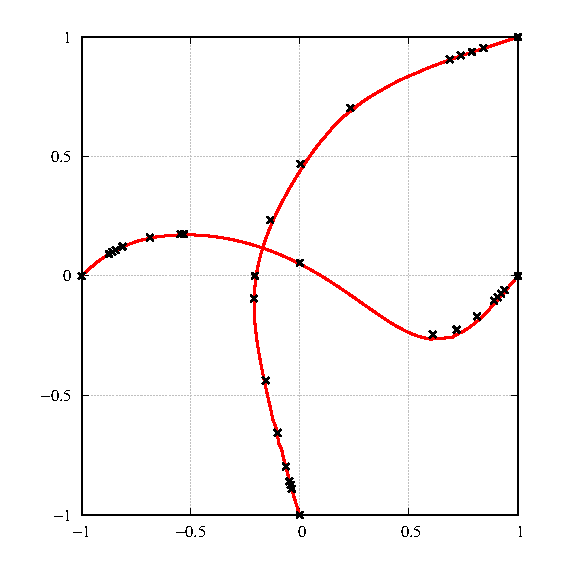
\includegraphics[scale=0.8,trim=0cm 0cm 0cm 0cm, clip=true]{Imagens/Cap4/cavidade_Re100.eps}}\\
	{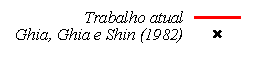
\includegraphics[scale=1.0,trim=0cm 0cm 0cm 0cm, clip=true]{Imagens/Cap4/legenda.pdf}}
	\caption{Cavidade 2D: Perfis de velocidade.} 
	\label{fig:cavidade_graficos_overlap}
\end{figure}

De acordo com os resultados obtidos, a metodologia se mostrou muito eficiente, com características promissoras para as próximas aplicações que serão realizadas neste projeto.
%
%\clearpage
%
%\textcolor{white}{ }


\end{document}
